\documentclass[a4paper, 10pt,notumble]{leaflet}
%Adjust paragraph indentation.
\setlength{\parindent}{0pt}
\setlength{\belowcaptionskip}{-20pt}

% Diagram for cover art
\usepackage{tikz}
\usetikzlibrary{shapes}
\usetikzlibrary{patterns}

\usepackage{caption}
\usepackage{array}
\usepackage{booktabs}

\usepackage[type={CC}, version={4.0}, modifier={by}]{doclicense} % Add text and icons for creative commons license

% Adjust formatting of list environments
\usepackage{enumitem}
\usepackage{calc}
\usepackage{multicol}

\setlist[itemize]{noitemsep, topsep=0pt, leftmargin=0.75cm, itemsep=\smallskipamount, labelindent=0.25cm}

\setlist[enumerate]{noitemsep, topsep=0pt, leftmargin=0.75cm, itemsep=\smallskipamount, labelindent=0.25cm}

\setlist[description]{noitemsep, topsep=0pt, labelindent=0.25cm, leftmargin=0.5cm, itemsep=\smallskipamount, font=\normalfont\bfseries}

\newlist{playerlist}{description}{1}
\newlist{playerlistnarrow}{description}{1}
\newlist{personadecklist}{description}{1}
\newlist{auxiliarydecklist}{description}{1}

\setlist[playerlist]{noitemsep, topsep=0pt, labelindent=0.25cm, leftmargin= 0.5cm,  labelsep=\widthof{\space}, font=\normalfont, labelwidth=\widthof{\redace\diamonds\ (The Student):\ }}

\setlist[playerlistnarrow]{noitemsep, topsep=0pt, labelindent=0.25cm, leftmargin= 0.5cm,  labelsep=\widthof{\space}, font=\normalfont\bfseries, labelwidth=\widthof{The Student:\ }}

\setlist[personadecklist]{noitemsep, topsep=0pt, labelindent=0.25cm, leftmargin= 0.5cm,  labelsep=\widthof{\space}, font=\normalfont\bfseries, labelwidth=\widthof{\textbf{Voting\ Cards\ \ (16)}}}

\setlist[auxiliarydecklist]{noitemsep, topsep=0pt, labelindent=0.25cm, leftmargin= 0.5cm,  labelsep=\widthof{\space}, font=\normalfont\bfseries, labelwidth=\widthof{\textbf{Challenge\ Cards\ \ (27)}}}

% Setting Fonts
\usepackage{fontspec}
%\setmainfont{XCharter}
\renewfontfamily\sectfont{Clarendon-Bold}

% Horrible hack to get small caps to work with Clarendon-Bold font.
\newcommand\fauxsc[1]{\fauxschelper#1 \relax\relax}
\def\fauxschelper#1 #2\relax{%
  \fauxschelphelp#1\relax\relax%
  \if\relax#2\relax\else\ \fauxschelper#2\relax\fi%
}
\def\fauxschelphelp#1#2\relax{%
  \ifnum`#1=\lccode`#1\relax\large{\char\uccode`#1}\else%
    \Large{#1}\fi%
  \ifx\relax#2\relax\else\fauxschelphelp#2\relax\fi}

% Macros for symbols that appear on playing cards
\newfontfamily\cardfont{Card Characters}[Scale=1.0]

\DeclareRobustCommand\spades[1][black]{\textcolor{#1}{\cardfont{\}}}}
\DeclareRobustCommand\hearts[1][red]{\textcolor{#1}{{\cardfont{\{}}}}
\DeclareRobustCommand\diamonds[1][red]{\textcolor{#1}{{\cardfont{[}}}}
\DeclareRobustCommand\clubs[1][black]{\textcolor{#1}{\cardfont{]}}}

\DeclareRobustCommand\two[1][black]{\textcolor{#1}{\cardfont{2}}}
\DeclareRobustCommand\three[1][black]{\textcolor{#1}{\cardfont{3}}}
\DeclareRobustCommand\four[1][black]{\textcolor{#1}{\cardfont{4}}}
\DeclareRobustCommand\five[1][black]{\textcolor{#1}{\cardfont{5}}}
\DeclareRobustCommand\six[1][black]{\textcolor{#1}{\cardfont{6}}}
\DeclareRobustCommand\seven[1][black]{\textcolor{#1}{\cardfont{7}}}
\DeclareRobustCommand\eight[1][black]{\textcolor{#1}{\cardfont{8}}}
\DeclareRobustCommand\nine[1][black]{\textcolor{#1}{\cardfont{9}}}
\DeclareRobustCommand\ten[1][black]{\textcolor{#1}{\cardfont{=}}}

\DeclareRobustCommand\jack[1][black]{\textcolor{#1}{\cardfont{J}}}
\DeclareRobustCommand\queen[1][black]{\textcolor{#1}{\cardfont{Q}}}
\DeclareRobustCommand\king[1][black]{\textcolor{#1}{\cardfont{K}}}
\DeclareRobustCommand\ace[1][black]{\textcolor{#1}{\cardfont{A}}}
%\DeclareRobustCommand\joker[1][black]{\textcolor{#1}{\cardfont{\textcolor{red}{J}\textcolor{black}{O}\textcolor{red}{K}\textcolor{black}{E}\textcolor{red}{R}}}}
\DeclareRobustCommand{\joker}[1][black]{\begin{tikzpicture}[baseline=-0.4em]
	\path[draw, semithick, #1] (0,0) circle (1.5mm);
	\path[#1, draw, fill=#1, rounded corners=0.1mm] (90:1.45mm) to (234:1.45mm) to (18:1.45mm) to (162:1.45mm) to (306:1.45mm) to cycle;%
\path (-2mm, 0) to (0mm, 0);
\end{tikzpicture}}%

\DeclareRobustCommand\redqueen[1][red]{\textcolor{#1}{\cardfont{Q}}}
\DeclareRobustCommand\redace[1][red]{\textcolor{#1}{\cardfont{A}}}

\newfontfamily\symbolfont{Noto Sans Symbols2}[Scale=1.75]
\DeclareRobustCommand\aceofspades{{\Huge{\symbolfont\symbol{"1F0A1}}}}
\DeclareRobustCommand\aceofhearts{{\Huge{\symbolfont\symbol{"1F0B1}}}}
\DeclareRobustCommand\aceofdiamonds{{\Huge{\symbolfont\symbol{"1F0C1}}}}
\DeclareRobustCommand\aceofclubs{{\Huge{\symbolfont\symbol{"1F0D1}}}}
\DeclareRobustCommand\jokercard{{\Huge{\symbolfont\symbol{"1F0CF}}}}

\tikzset{spadescard/.pic={
	\node[draw, thick, minimum height=12.25mm, minimum width=8.75mm, rounded corners=1mm] (border) at (0,0) {};
	\node (suit) at (0,0) {\Large{#1}};
	\node (ul) at (-2.75mm, 4mm) {\spades};
	\node[rotate=180] (br) at (2.75mm, -4mm) {\spades};
}}

\tikzset{heartscard/.pic={
	\node[draw, thick, minimum height=12.25mm, minimum width=8.75mm, rounded corners=1mm] (border) at (0,0) {};
	\node (suit) at (0,0) {\Large{#1}};
	\node (ul) at (-2.75mm, 4mm) {\hearts};
	\node[rotate=180] (br) at (2.75mm, -4mm) {\hearts};
}}

\tikzset{clubscard/.pic={
	\node[draw, thick, minimum height=12.25mm, minimum width=8.75mm, rounded corners=1mm] (border) at (0,0) {};
	\node (suit) at (0,0) {\Large{#1}};
	\node (ul) at (-2.5mm, 4.2mm) {\clubs};
	\node[rotate=180] (br) at (2.5mm, -4.2mm) {\clubs};
}}

\tikzset{diamondscard/.pic={
	\node[draw, thick, minimum height=12.25mm, minimum width=8.75mm, rounded corners=1mm] (border) at (0,0) {};
	\node (suit) at (0,0) {\Large{#1}};
	\node (ul) at (-2.75mm, 4mm) {\diamonds};
	\node[rotate=180] (br) at (2.75mm, -4mm) {\diamonds};
}}

\tikzset{dottedcardoutline/.pic={
	\node[draw, dotted, very thick, minimum height=12.25mm, minimum width=8.75mm, rounded corners=1mm] (border) at (0,0) {};
}}

\tikzset{head/.pic={
	\node (A) at (0,0) {
\includegraphics[scale=0.06]{head_outline_filled.png}};
	\node (B) at (1.1,0.95) {\fontsize{60}{72}{\hearts}};
	\node (B) at (-1.9,0.95) {\fontsize{60}{72}{\diamonds}};
	\node (B) at (-0.475,2.6) {\fontsize{60}{72}{\spades}};
	\node (B) at (-0.475,-0.4) {\fontsize{60}{72}{\clubs}};
}}


\tikzset{cardback/.pic={
	\node[draw, thick, minimum height=12.25mm, minimum width=8.75mm, rounded corners=1mm, pattern=crosshatch, pattern color=blue] (border) at (0,0) {};
	\pic[scale=0.095, transform shape] at (0,0) {head};

}}


\usepackage[hidelinks]{hyperref} % Add hyperlinks to the pdf file. This should usually be the last package loaded before \begin{document}

% Start Document

\begin{document}
% Cover page with title, cover art, description, and author
\center{\setmainfont{XCharter}}
{\footnotesize{Version 0.1}}
\setmainfont[Scale=2.8]{Clarendon-Bold}
\begin{center}
\begin{tabular}{c@{\hspace{0.25ex}}l@{\hspace{0.05ex}}c@{\hspace{0.25ex}}l}
\huge{H} & \huge{\textcolor{red}{E}} & \huge{A} & \huge{\textcolor{red}{D}} \\[0.5ex]
\huge{\textcolor{red}{T}} & \huge{R} & \huge{\textcolor{red}{I}} & \huge{P}
\end{tabular}
\end{center}

\vfill

\begin{figure}[h]
\centering
	\begin{tikzpicture}
	\node (A) at (0,0) {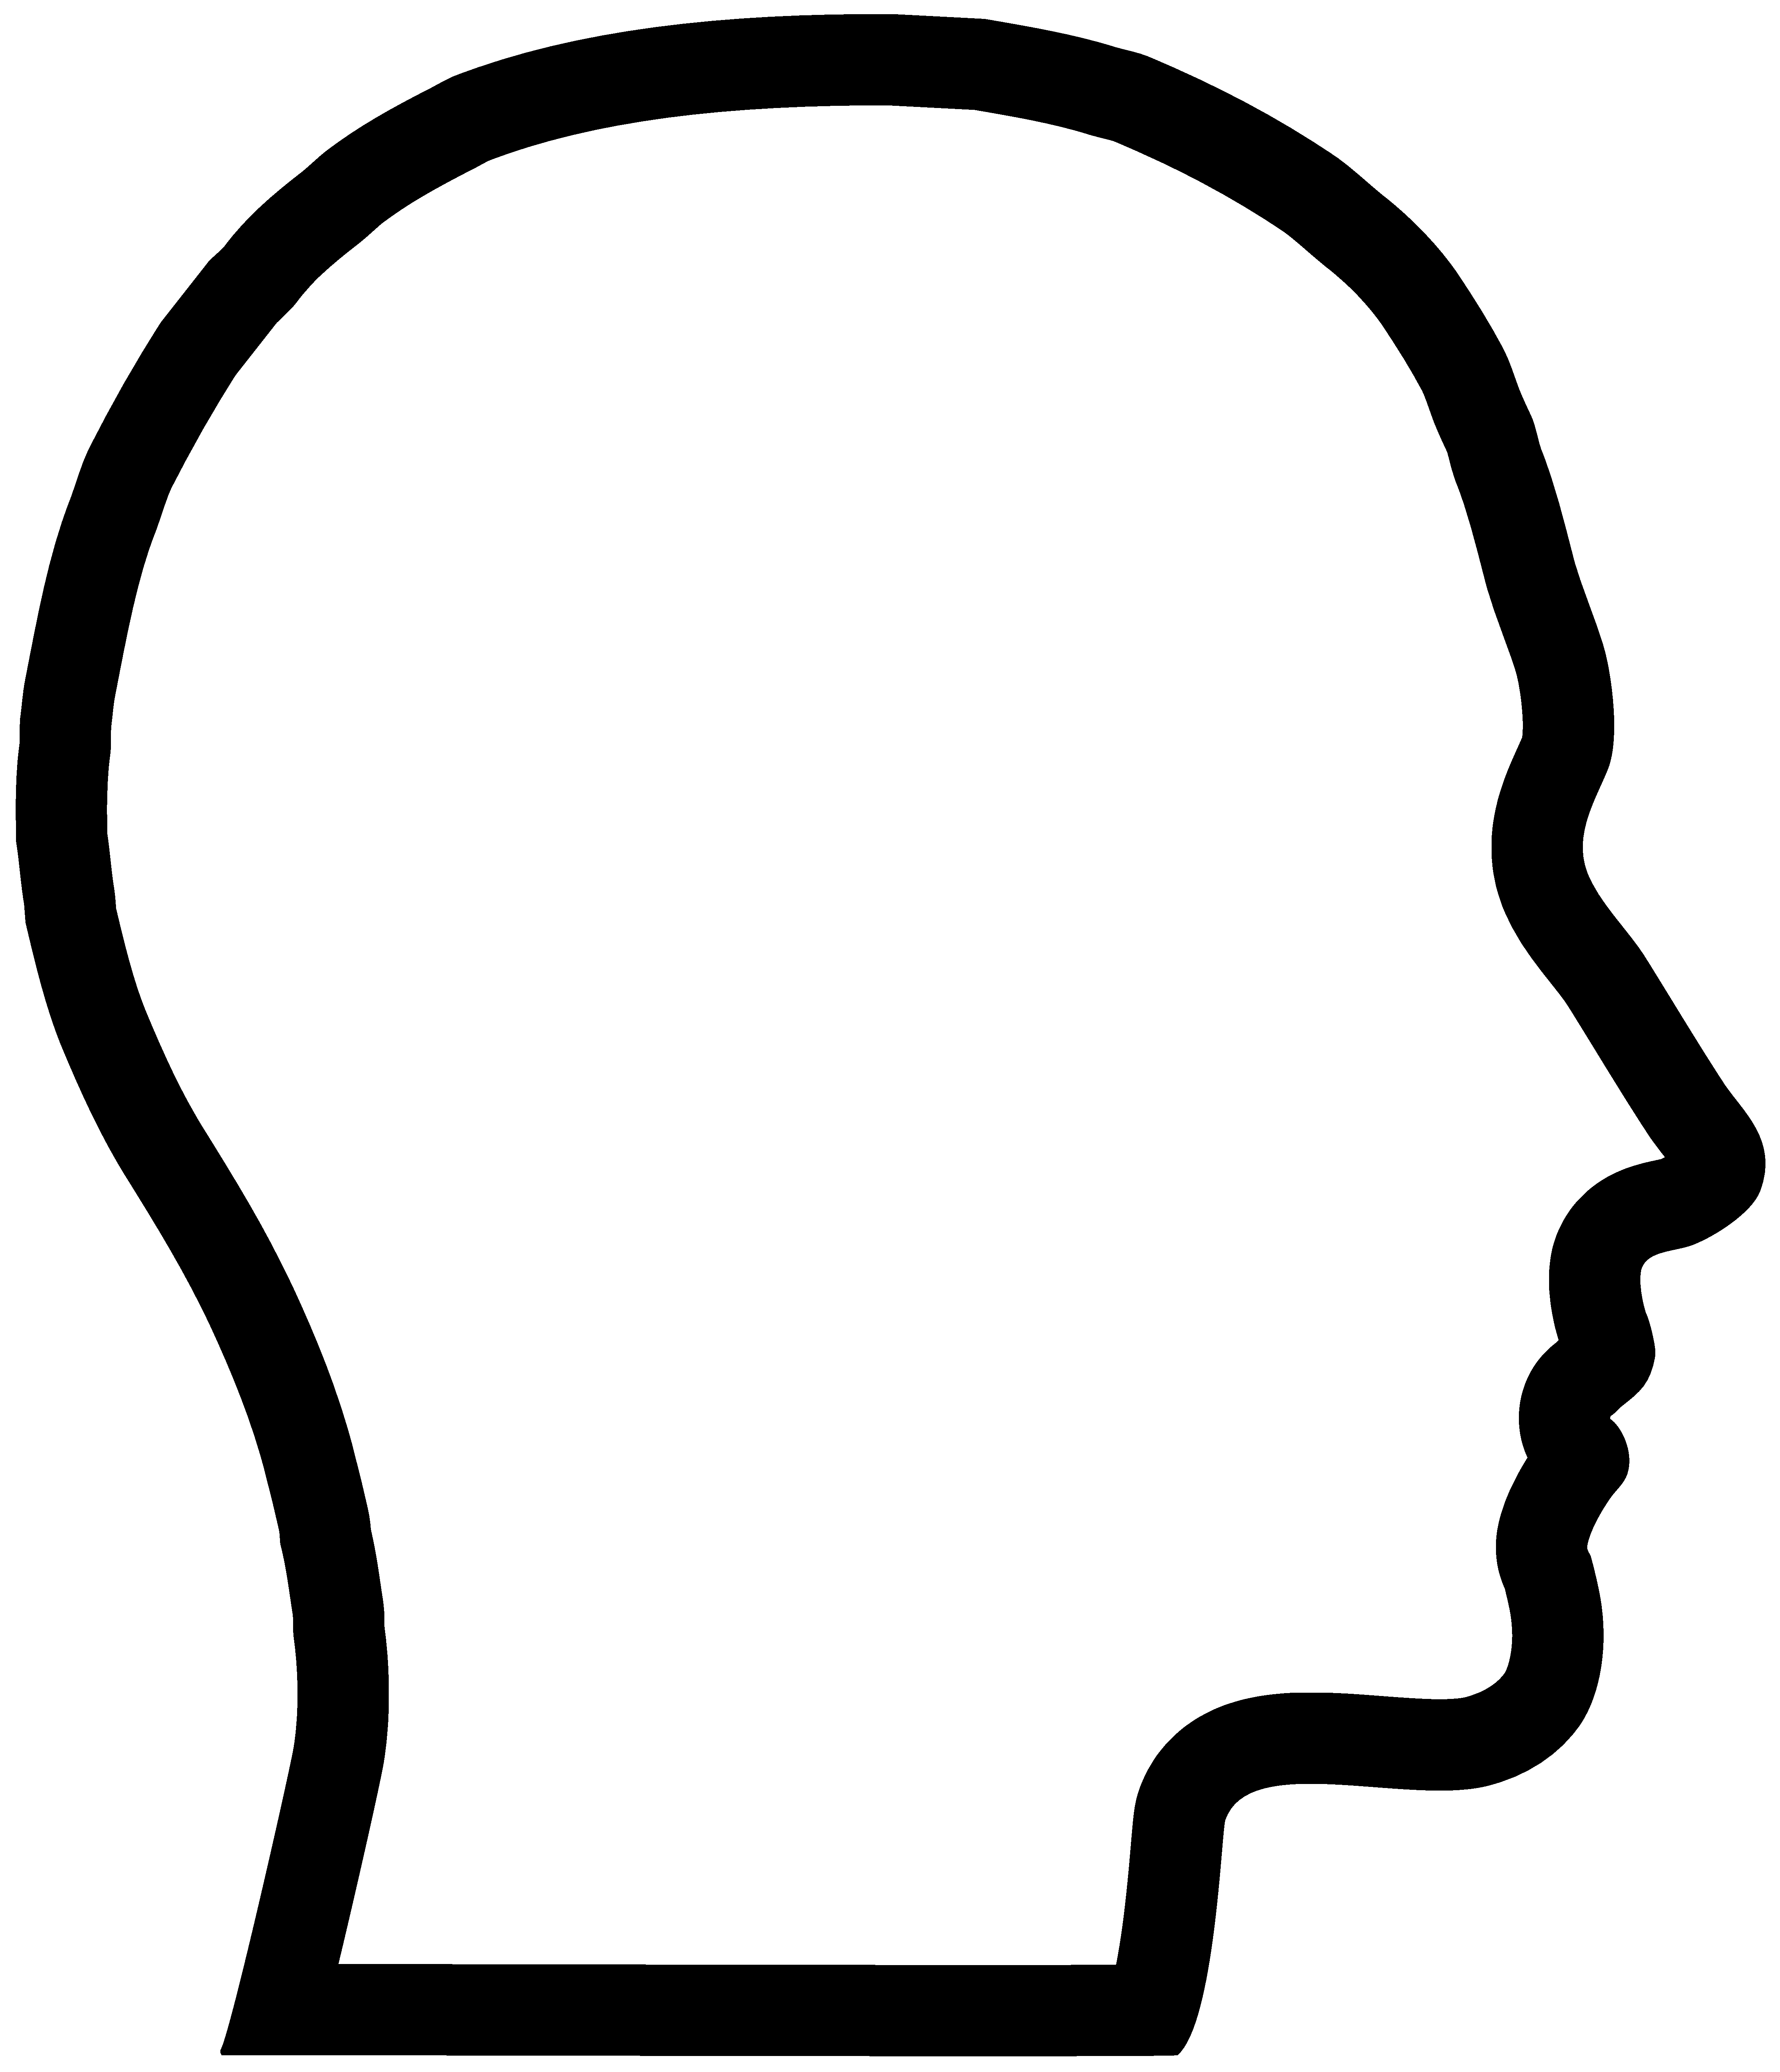
\includegraphics[scale=0.06]{head_outline.png}};
	\node (B) at (1.1,0.95) {\fontsize{60}{72}{\hearts}};
	\node (B) at (-1.9,0.95) {\fontsize{60}{72}{\diamonds}};
	\node (B) at (-0.475,2.6) {\fontsize{60}{72}{\spades}};
	\node (B) at (-0.475,-0.4) {\fontsize{60}{72}{\clubs}};
	\end{tikzpicture}
\end{figure}

\vfill

\setmainfont[Scale=1.5]{XCharter}
\begin{center}
A card game for four players

\smallskip

designed by Michael Purcell
\end{center}

\newpage

\setmainfont{XCharter}
\raggedright
\section{Overview}
{\setmainfont{Clarendon-Light} HEAD TRIP} is a game for four players that is played with two decks of cards. During the game, each player will portray an \emph{aspect} of the personality of a teenage boy named Bobby.
\begin{playerlist}
	\item[\jack\clubs\ (The Animal):] represents Bobby's physicality.
	\item[\redqueen\hearts\ (The Angel):] represents Bobby's compassion.
	\item[\king\spades\ (The Genius):] represents Bobby's intellect.
	\item[\redace\diamonds\ (The Student):] represents Bobby's curiosity.
\end{playerlist}

Only one aspect can control Bobby's actions at any given time. That aspect is called the \emph{pilot}.
So, the players will have to compete for control as Bobby faces a series of challenges.

To determine the outcome of each challenge, the pilot will add a card to the \emph{tableau}. The outcome of the challenge is determined by the rank of that card. 
 
There are three types of challenges: \clubs\ (physical), \hearts~(social), and \spades\ (mental). Different aspects receive different rewards when Bobby succeeds or fails at the various types of challenges.


The players with the highest scores at the end of the game are the winners.

\subsection{The Cards}
The \emph{persona deck} is a complete (54 cards) standard deck of playing cards. It consists of:
\begin{personadecklist}
	\item[Action Cards\hfill\normalfont{(36):}] all \two\ \textendash\ \ten\ cards.
	\item[Voting Cards\hfill\normalfont{(16):}] all \jack, \queen, \king, \ace\ cards.
	\item[Recall Cards\hfill\normalfont{(2):}] all \joker\ (joker) cards.
\end{personadecklist}

The \emph{auxiliary deck} is a subset (34 cards) of a standard deck of cards. It consists of:
\begin{auxiliarydecklist}
	\item[Challenge Cards\hfill\normalfont{(27):}] \two\ \textendash\ \ten\ of \clubs, \hearts, \spades.
	\item[Aspect Cards\hfill\normalfont{(4):}] \jack\clubs, \queen[red]\hearts[red], \king\spades, \ace[red]\diamonds[red].
	\item[Label Cards\hfill\normalfont{(3):}] \ace\clubs, \ace[red]\hearts, \ace\spades.
\end{auxiliarydecklist}

It may be useful to use decks with different coloured backs or decks of different sizes to make it easier to see which cards belong to each deck.

\newpage

\subsection{The Tableau}
The tableau represents Bobby's long-term memory.
It is the part of the play area where the pilot plays an action card when Bobby faces a challenge.
It consists of three rows of cards, one for each type of challenge.

At the beginning of the game, the tableau is empty. A label card is used to indicate the position of the start of each row as in the following diagram:
%\smallskip
\begin{figure}[h]\centering
\begin{tikzpicture}[scale=0.9]
	\pic[rotate=90, transform shape] () at (0,32mm) {clubscard={\ace}};
	\pic () at (15mm, 32mm) {dottedcardoutline};
	\pic () at (27mm, 32mm) {dottedcardoutline};
	\pic () at (39mm, 32mm) {dottedcardoutline};
	\pic () at (51mm, 32mm) {dottedcardoutline};
	\node[draw, fill=black, circle, inner sep=0.5pt] () at (59mm,32mm) {};
	\node[draw, fill=black, circle, inner sep=0.5pt] () at (61mm,32mm) {};
	\node[draw, fill=black, circle, inner sep=0.5pt] () at (63mm,32mm) {};

	\pic[rotate=90, transform shape] () at (0,16mm) {heartscard={\redace}};
	\pic () at (15mm, 16mm) {dottedcardoutline};
	\pic () at (27mm, 16mm) {dottedcardoutline};
	\pic () at (39mm, 16mm) {dottedcardoutline};
	\pic () at (51mm, 16mm) {dottedcardoutline};
	\node[draw, fill=black, circle, inner sep=0.5pt] () at (59mm,16mm) {};
	\node[draw, fill=black, circle, inner sep=0.5pt] () at (61mm,16mm) {};
	\node[draw, fill=black, circle, inner sep=0.5pt] () at (63mm,16mm) {};

	\pic[rotate=90, transform shape] () at (0,0) {spadescard={\ace}};
	\pic () at (15mm, 0) {dottedcardoutline};
	\pic () at (27mm, 0) {dottedcardoutline};
	\pic () at (39mm, 0) {dottedcardoutline};
	\pic () at (51mm, 0) {dottedcardoutline};
	\node[draw, fill=black, circle, inner sep=0.5pt] () at (59mm,0) {};
	\node[draw, fill=black, circle, inner sep=0.5pt] () at (61mm,0) {};
	\node[draw, fill=black, circle, inner sep=0.5pt] () at (63mm,0) {};
\end{tikzpicture}
\caption*{An empty tableau.}
\end{figure}

\bigskip
During the game, cards will be added to the tableau.
At the end of the game, the state of the tableau will be used to compute the players' scores.

\section{Set Up}
To prepare to play the game the players should:
\begin{enumerate}
\item Place the label cards face up in the middle of the play area to indicate the location of the tableau.
\item Shuffle the challenge cards and place them face down near the tableau.
\item Deal an aspect card to each player. The players should place their aspect cards face up in the play area in front of themselves.
\item Collect all of the voting cards of the same suit as their aspect cards. The players should place their voting cards face down near their aspect card.
\item Collect all of the action cards of the same suit as their aspect cards.
\item Place the recall cards face up near the tableau. 
\end{enumerate}
The Student is the starting pilot.

\newpage

\section{Game Play}
The game takes place over a sequence of rounds.
During each round:
\begin{enumerate}
	\item The pilot must reveal the next challenge card. 
	\item The pilot may step down. If two or more players agree to do so, they may spend a recall card to force the pilot to step down.
	\item If the pilot stepped down, then the players must elect a new pilot.
	\item The pilot must play an action card. 
\end{enumerate}
The game ends when any player plays their last action card or after Bobby faces the last challenge.

\subsection{Playing an Action Card}
The pilot must add one action card to the tableau.
If the rank of the pilot's card meets or exceeds the rank of the challenge card, then Bobby succeeds. Otherwise, Bobby fails.

The pilot's card is added to the tableau in the row corresponding to the suit of the challenge card. If Bobby succeeds, then the pilot's card is played face up.  Otherwise, their card is played face down. 

\subsection{Electing a Pilot}
Each player must vote for an aspect by turning their corresponding voting card face up.
The aspect who receives the most votes wins the election. 

In the case of a tie, The Student must decide which of the leading vote-getters wins the election. 

The winner of the election must become the new pilot.

\subsection{Scoring}
The score for each player is given by:
\begin{playerlistnarrow}
	\item[\normalfont{The Animal:}] total physical successes.
	\item[\normalfont{The Angel:}] total social successes.
	\item[\normalfont{The Genius:}] total mental successes.
	\item[\normalfont{The Student:}] total failures.
\end{playerlistnarrow}
The players with the highest scores win the game.
\newpage



\section{Example of Play}
The following is a description of a single round of play. The~Genius is the current pilot.

\begin{enumerate}
	\item The Genius reveals the next challenge card is \four[red]\hearts.
	\item The Genius decides to stand down.
	\item The players cast their votes for which aspect should become the next pilot. The votes are:
%\begin{playerlistnarrow}
%\smallskip
%	\item[\normalfont{The Animal:}] \jack\clubs
%	\item[\normalfont{The Angel:}] \queen[red]\hearts
%	\item[\normalfont{The Genius:}] \jack\spades
%	\item[\normalfont{The Student:}] \jack[red]\diamonds
%\end{playerlistnarrow}
%\smallskip
	\begin{table}[h]
	\centering
	\begin{tabular}{l r}
	\toprule
	Aspect & Vote \\ \midrule
	The Animal & \jack\clubs \\
	The Angel  & \queen[red]\hearts \\
	The Genius & \jack\spades \\
	The Student & \jack[red]\diamonds \\ \bottomrule
	\end{tabular}
	\end{table}
%	
%	\begin{figure}[h]
%	\centering
%	\begin{tikzpicture}[scale=0.9]
%		\pic () at (0,0) {clubscard={\jack}};
%		\pic () at (22.5mm,0) {heartscard={\queen[red]}};
%		\pic () at (45mm,0) {spadescard={\jack}};
%		\pic () at (67.5mm,0) {diamondscard={\jack[red]}};
%		\node[label=below:{The Animal}, minimum height=12.25mm, minimum width=8.75mm] () at (0,0) {};
%		\node[label=below:{The Angel}, minimum height=12.25mm, minimum width=8.75mm] () at (22.5mm,0) {};
%		\node[label=below:{The Genius}, minimum height=12.25mm, minimum width=8.75mm] () at (45mm,0) {};
%		\node[label=below:{The Student}, minimum height=12.25mm, minimum width=8.75mm] () at (67.5mm,0) {};
%
%	\end{tikzpicture}
%	\end{figure}
	
	That is, The Animal receives three votes and The~Angel receives one vote. So, The Animal will be the next pilot.
	\item The Animal decides to play \five\clubs, which he adds face up to the middle row of the tableau. This yields the partially-completed tableau:
	
\begin{figure}[h]\centering
\begin{tikzpicture}[scale=0.9]
	\pic[rotate=90, transform shape] () at (0,32mm) {clubscard={\ace}};
	\pic () at (15mm, 32mm) {diamondscard={\six[red]}};
	\pic () at (27mm, 32mm) {spadescard={\eight}};
	\pic () at (39mm, 32mm) {cardback};

	\pic[rotate=90, transform shape] () at (0,16mm) {heartscard={\redace}};
	\pic () at (15mm, 16mm) {cardback};
	\pic () at (27mm, 16mm) {heartscard={\seven[red]}};
	\pic () at (39mm, 16mm) {heartscard={\five[red]}};
	\pic () at (51mm, 16mm) {clubscard={\five}};

	\pic[rotate=90, transform shape] () at (0,0) {spadescard={\ace}};
	\pic () at (15mm, 0) {clubscard={\eight}};
	\pic () at (27mm, 0) {cardback};
\end{tikzpicture}
\caption*{A partially-completed tableau.}
\end{figure}

\bigskip
After this round The Student and The~Angel both have three points, The Animal has two points, and The Genius has one point.

\end{enumerate}

%\subsection{Boss Battle}
%The players can agree to have Bobby face an additional challenge at the end of the game. If Bobby fails this final challenge, then none of the players score any points and no one can win the game.
%
%When facing this final challenge, however, all of the aspects may contribute an action card.
%
%If the sum of the contributed cards meets or exceeds the rank of the final challenge card, then Bobby succeeds. Otherwise, Bobby fails.
%
%The players should use the next challenge card for Bobby to face as the final challenge. If the basic game ended because Bobby faced the last challenge, then the players should choose a random challenge card for Bobby to face as the final challenge.
%
%If the basic game ended because a player ran out of action cards, then that player will not be able to contribute to the final challenge.



%
%\subsection{Asymmetric Powers}
%Test
%
%\subsection{Boss Battle}
%Test
%
\newpage
\section{Variants}
There are several variants of the basic game that experienced players may want to explore. These variants add some additional complexity to the game and allow for more strategic play.

\subsection{Multi-game Sessions}
The players can agree to play several games in a single session and combine their scores in the individual games to compute a single overall \emph{session score}.

Each player's session score is the sum of the player's scores in the individual games. The players with the highest session scores win.
	
\subsection{Aspect Affinities} 
The players can agree to allow players to add two cards to the tableau when the suit of the challenge card matches that of the pilot.

If the sum of the ranks of the two cards meets or exceeds the rank of the challenge card, then Bobby succeeds. Otherwise, Bobby fails.

\section{Acknowledgements}
%The design of {\setmainfont{Clarendon-Light}{HEAD TRIP}} has been vastly improved by the influence of ideas and mechanics from other games and the feedback provided by playtesters.
%
%\subsection{Contributors}
The following people made significant contributions throughout the design process:
\vspace{-1.75ex}
\begin{multicols}{2}
\begin{itemize}[itemsep=0pt, topsep=0pt, partopsep=0pt]
%  \item Keydan Bruce
%  \item Farzana Choudhury
%  \item Michael Cromer
  \item Dannielle Harden
  \item Andrew Hellyer
%  \item Sarah Hewat
%  \item Scott Joblin
  \item David McKenzie
  \item Paul Murray
  \item Kira Purcell
  \item Luke Purcell
%  \item Will Purcell
%  \item Jo Stephenson
%  \item Brett Witty
\end{itemize}
\end{multicols}

%\subsection{Influences}
%The theme of {\setmainfont{Clarendon-Light} HEAD TRIP} was strongly influenced by several icons of popular culture. These include:
%\begin{description}
%	\item[Inside Out\normalfont{:}] A feature-length animated Pixar film that was released in 2015.
%	\item[Herman's Head\normalfont{:}] A television series that aired on the Fox television network from 1991 to 1994.
%	\item[Cranium Command\normalfont{:}] An attraction at Walt Disney World's Epcot theme park from 1989 to 2007.
%\end{description}
%
%The idea of players portraying the various aspects of a character's personality in a game has is also well established. Notable examples include:
%\begin{description}
%	\item[Everyone is John\normalfont{:}] A competitive roleplaying game created by Michael B. Sullivan in 2002.
%	\item[Bluebeard's Bride\normalfont{:}] An investigatory horror roleplaying game created by Marissa Kelly in 2017. 
%\end{description}

\subsection{Design Tools}
The following tools were used to create this leaflet:
\begin{description}[itemsep=0pt]
	\item[XeLaTeX:] Typesetting and layout.
	\item[TikZ:] Diagrams and art.
\end{description}
The fonts used herein are Clarendon and Charter.

\textbf{Contact}: \href{mailto:head.trip.card.game@gmail.com}{head.trip.card.game@gmail.com}

\medskip
\begin{tabular}{@{}m{\textwidth-\widthof{\Huge{\doclicenseIcon}}}@{}m{\widthof{\Huge{\doclicenseIcon}}}@{}}
\footnotesize{This work is licensed under a Creative Commons\newline ``Attribute 4.0 International'' license.} & \Huge{\doclicenseIcon} \\
\end{tabular}
%\section{Acknowledgements}
%Test
%
\end{document}